\section{Results}\label{sec:results}

%Här kan du till exempel presentera resultat av experiment, bevis, analys av data etc. Dina resultat måste beskrivas så tydligt att en läsare kan bedöma dem.  Du ska också förklara och analysera resultaten.

The results so far is divided up in two relevant subsections where the first handles the input inference test and the second handles the 3D reconstruction using \aruco corners.
\subsection{OpenPose output inference results}%
\label{sub:res:op_inference}
Using \openpose{ } on a human subject that is located on the ground can provide diverse results dependent on the relative rotation of the body the camera.
How well does it preform when the subject is laying such as in image North in figure~\ref{fig:camera_pos_lables}.
And how is the preference for each label in the \operpose{ } data set against a human labler.

During statistical tests with F/T-test the degrees of freedom will tell you how many data points there is behind the results.
Thus can be shown in table~\ref{tab:results:degfreedom} the degrees of freedom for each label can be found.
While table~\ref{lab:results:human_vs_openpose} shows the degrees of freedom dependent on direction where the camera was located.

From the results in table~\ref{tab:results:human} and table~\ref{lab:results:human_lable} it can be observed that F-test is mostly rejected while the T-test is mostly reported as accept.
This then propose that the $H_0$ hypothesis is weekly rejected as it fails on $\sigma_H = \simgma_O$ but is passed on $\mu_H = \mu_O$.
There fore the $H_1$ hypotheses is accepted and that shows that \openpose{ } do not have same accuracy as an human label setter.



%----------------------------
\begin{table}[htb]
    \begin{center}
    \begin{minipage}{0.4\textwidth}
        \begin{center}
            \input{../results/error_degdf_df.latex}
        \end{center}
        \caption[Degrees of freedom human vs openpose]{The degrees of freedom for human and \openpose is due to the quite limited dataset not in most cases not statistically viable but perhaps it cold work as a marker.}
        \label{tab:results:degfreedom}
    \end{minipage}
    \begin{minipage}{0.4\textwidth}
        \begin{center}
            \input{../results/direction_degdf_df.latex}
        \end{center}
        \caption[Directional degrees of freedom]{The directional degrees of freedom is a bit better because it do not care about the labels, just the total error for that direction. }
        \label{tab:results:dirdegfreedom}
    \end{minipage}
    \end{center}
\end{table}
%----------------------------
\begin{table}[htb]
    \begin{center}
        \input{../results/ftest_pos_df.latex}
    \end{center}
    \caption{The directional results from F-test and T-test}
    \label{lab:results:human_lable}
\end{table}
%----------------------------
\begin{table}[htb]
    \begin{center}
        \input{../results/error_df.latex}
    \end{center}
    \caption[Results in image domain]{The error results for the human vs \openpose in the image domain. Observe the large variance in the forth column that suggests that \openpose have problem finding the correct solution for that label. It can also be observed that the half of the data in comparison with the human is missing from \openpose columns thus indicating again that it could not find a solution to that label.}
    \label{lab:results:human_vs_openpose}
\end{table}
%----------------------------
\begin{table}[htb]
    \begin{center}
        \input{../results/ftest_pds.latex}
    \end{center}
    \caption{Datasets}
    \label{tab:results:human}
\end{table}


\subsection{3D reconstruction using Aruco}%
Reconstruction of the sparce 3D map done by using \aruco{'s} in a pose quiver without solving the bundle adjustment problem was attempted to be solved.
The method derived relied on Dijkstra algorithm and cumulative transfer poses from corner to corner to camera.
An then by solving the epee polar geometry a point cloud is supposed to be generated.
How ever the due to the cumulative output of the algorithms the positions of the camera is never reaching a satisfiable position.



\label{sub:res:3drec}
\begin{figure}
\begin{center}
    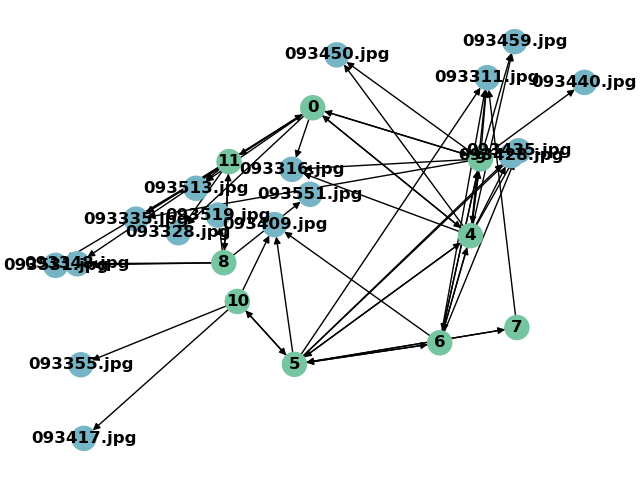
\includegraphics[scale=0.6]{results/atlas.png}
\end{center}
\caption[Results from camera mapping]{Reconstructing the camera pose from the images using Dijkstras algorithm  data proved to be a harder problem then initially thought. Ni this results the green numbered nodes seams to find the correct location, but the input camera view nodes in blue do not.}
\label{fig:results:mapreconstruction}
\end{figure}


